\documentclass[11pt,a4paper]{article}
\usepackage[T1]{fontenc}
\usepackage[utf8]{inputenc}
\usepackage{lmodern}
\usepackage[margin=27mm]{geometry}
\usepackage{amsmath,amssymb,amsthm,bm}
\usepackage{graphicx,booktabs,microtype,float,needspace}
\usepackage[numbers,sort&compress]{natbib}
\usepackage[colorlinks=true,linkcolor=blue,citecolor=blue,urlcolor=blue]{hyperref}
\usepackage[section]{placeins}
\hypersetup{pdftitle={Exact local spectrum and a residual-rate obstruction for quantum Latin-square normalization},pdfauthor={Xiaojian Zeng},pdfkeywords={quantum Latin square, polar normalization, tangent spectrum}}
\newtheorem{proposition}{Proposition}
\newtheorem{lemma}{Lemma}
\newcommand{\C}{\mathbb C}
\newcommand{\R}{\mathbb R}
\newcommand{\Id}{I_4}
\newcommand{\adj}{^{\dagger}}
\newcommand{\fro}[1]{\left\|#1\right\|_{\mathrm F}}
\newcommand{\TR}{T_{\mathcal R}}
\newcommand{\TC}{T_{\mathcal C}}
\DeclareMathOperator{\Tr}{Tr}
\DeclareMathOperator{\diag}{diag}
\DeclareMathOperator{\spec}{spec}
\title{Exact local spectrum and a residual-rate obstruction\texorpdfstring{\\}{ }for quantum Latin-square normalization}
\author{Xiaojian Zeng\\[2pt]
\small PBC School of Finance, Tsinghua University\\
\small Beijing 100190, China\\
\small \texttt{xiaojianzeng@foxmail.com}}
\date{}
\begin{document}
\maketitle

\begin{abstract}
Alternating row and column normalization provides a numerical constructor for quantum Latin squares and rank-one quantum permutation matrices. We compute the complete real tangent spectrum of one normalization cycle at an explicit one-parameter family of order-four quantum Latin squares. On the 64-dimensional column-unitary tangent space, the eigenvalues are $0$, $1$, $(1+\cos\theta)/2$ and $(1-\cos\theta)/2$, with multiplicities $16$, $32$, $8$ and $8$, respectively, combining at exceptional parameters. A direct block decomposition proves the formula for every real parameter. We then connect a nonneutral eigenvector to the maximum row Frobenius residual used by the constructor. For any prescribed factor below one, any tolerance on the eight inverted Gram spectra, and any neighbourhood size, an exactly column-unitary input has a one-cycle residual ratio above that factor while all inverted Grams remain within the tolerance of the identity. Thus excellent Gram conditioning cannot guarantee uniform strict one-cycle progress. The result gives an explicit local benchmark; it does not establish nonlinear convergence, failure probabilities or almost-sure arbitrary-precision termination.
\end{abstract}

\noindent\textbf{Keywords:} quantum Latin square; quantum permutation matrix; polar normalization; alternating projections; tangent spectrum

\section{Introduction}

A quantum Latin square is an array of vectors for which every row and every column is an orthonormal basis. Such arrays connect quantum combinatorial constructions with unitary error bases \cite{MustoVicary2016}. Their rank-one projections form quantum permutation matrices. Alternating normalization is a practical way to seek these arrays: one makes the rows orthonormal, then the columns, and repeats. The rank-one quantum Sinkhorn procedure of Nechita, Schmidt and Weber \cite{NechitaSchmidtWeber2023} uses principal inverse square roots of the row and column Gram matrices. Its almost-sure finite termination at each fixed accuracy is posed as Conjecture 3.2 of the specified preprint version. A later discussion again lists convergence as a problem \cite[Problem 3.13]{Weber2023}.

The local geometric mechanism is familiar. Near a common point of two smooth constraint manifolds, the derivative of an alternating projection is a product of their tangent projectors \cite{LewisMalick2008}. Small angles can produce slow linearized progress. Applying this observation to a particular quantum constructor still requires the tangent spectrum, its multiplicities and its relation to the residual actually monitored by the algorithm. Moreover, a well-conditioned inverse square root and a favourable angle between constraints are different requirements.

Here we give that calculation for an explicit order-four block-rotation family. The contribution is the full family-specific spectrum and a legal perturbation witnessing nonuniform one-cycle progress in the source residual. The family construction and the general projection-angle mechanism are not novelty claims. Our result makes no nonlinear or global convergence assertion. It supplies a concrete benchmark for implementations and shows why a conditioning monitor alone cannot imply a parameter-independent strict one-cycle residual factor.

\section{Constructor, residual and an exact family}
\label{sec:model}

All indices run from $0$ to $3$. An array $x=(x_{ij})$ has entries in $\C^4$. Its row and column square matrices are
\begin{equation}
 A_i(x)=[x_{i0}\ x_{i1}\ x_{i2}\ x_{i3}],\qquad
 U_j(x)=[x_{0j}\ x_{1j}\ x_{2j}\ x_{3j}].
 \label{eq:squares}
\end{equation}
Write $\mathcal R$ and $\mathcal C$ for arrays with all $A_i$ and all $U_j$ unitary, respectively. Each is a product of four copies of $U(4)$, of real dimension $64$, embedded in the real Euclidean space
\begin{equation}
 \mathcal E=(\C^4)^{4\times4},\qquad
 \langle H,G\rangle_{\R}=\operatorname{Re}\sum_{i,j}H_{ij}\adj G_{ij},
 \label{eq:metric}
\end{equation}
of dimension $128$. The array norm is $\fro{x}^2=\sum_{i,j}x_{ij}\adj x_{ij}$.

One full source cycle $F$ is the row-then-column map
\begin{equation}
\begin{aligned}
 R_i(x)&=\sum_jx_{ij}x_{ij}\adj,
 &y_{ij}&=R_i(x)^{-1/2}x_{ij},\\
 C_j(y)&=\sum_i y_{ij}y_{ij}\adj,
 &F(x)_{ij}&=C_j(y)^{-1/2}y_{ij}.
\end{aligned}
 \label{eq:cycle}
\end{equation}
Every inverse square root is the positive Hermitian one; a cycle is defined only if its four $R_i$ and four $C_j$ are positive definite. For a nonsingular square $A=V\Sigma W\adj$,
\begin{equation}
 (AA\adj)^{-1/2}A=VW\adj.
 \label{eq:polar}
\end{equation}
This is the nearest-unitary polar factor, so locally $F=P_{\mathcal C}P_{\mathcal R}$. It is the same defining normalization, not a QR replacement. After column normalization the column Grams are exactly the identity in exact arithmetic. The source stopping observable is therefore the maximum row Hilbert--Schmidt, or Frobenius, defect
\begin{equation}
 e(x)=\max_i\fro{R_i(x)-\Id},\qquad x\in\mathcal C.
 \label{eq:residual}
\end{equation}
The trace in this norm is unnormalized. Vector entries, defects and iteration counts are dimensionless. The map is a classical numerical constructor, with no physical time or spatial boundary condition.

Let $c=\cos\theta$, $s=\sin\theta$, and set $u=c e_0+s e_1$, $v=-s e_0+c e_1$ in the computational basis of $\C^4$. We study
\begin{equation}
 Q(\theta)=
 \begin{pmatrix}
 e_0&e_1&e_2&e_3\\
 e_1&e_0&e_3&e_2\\
 e_2&e_3&u&v\\
 e_3&e_2&v&u
 \end{pmatrix}.
 \label{eq:family}
\end{equation}
Since $\langle u,v\rangle=0$ and $\|u\|=\|v\|=1$, every row and column is an orthonormal basis. Hence $Q(\theta)\in\mathcal R\cap\mathcal C$ and $F(Q(\theta))=Q(\theta)$ for every real $\theta$. This elementary family is used only to analyze the iterator; no new construction or equivalence classification is asserted.

\Needspace{12\baselineskip}
\section{Complete tangent spectrum}
\label{sec:spectrum}

\begin{proposition}
\label{prop:spectrum}
For the family \eqref{eq:family}, let $D_\theta$ be the real derivative $DF(Q(\theta))$ restricted to $\TC(Q(\theta))$. Its characteristic polynomial is
\begin{equation}
 \det(zI-D_\theta)=z^{16}(z-1)^{32}
 \left(z-\frac{1+c}{2}\right)^8
 \left(z-\frac{1-c}{2}\right)^8.
 \label{eq:charpoly}
\end{equation}
Multiplicities combine whenever roots coincide. At $\theta=0\pmod\pi$, the spectrum is $0$ with multiplicity $24$ and $1$ with multiplicity $40$. At $c=0$, it is $0$, $1/2$, $1$ with multiplicities $16$, $16$, $32$.
\end{proposition}

We first recover the standard tangent-projector formula directly from the source map. At a unitary square $A$, in a real perturbation direction $H$,
\begin{align}
 [(A+hH)(A+hH)\adj]^{-1/2}(A+hH)
 &=A+\frac h2(H-AH\adj A)+O(h^2).
 \label{eq:derivative}
\end{align}
Indeed, the Gram matrix is $I+h(HA\adj+AH\adj)+O(h^2)$ and the derivative of its principal inverse square root at $I$ is minus one half of that Hermitian perturbation. Thus
\begin{equation}
 L_A(H)=\tfrac12(H-AH\adj A)
 \label{eq:projector}
\end{equation}
is the real orthogonal projector onto $T_AU(4)=\{AK:K\adj=-K\}$. Applying it to all rows or columns gives $L_{\mathcal R}$ and $L_{\mathcal C}$. On the column tangent space,
\begin{equation}
 D_\theta=L_{\mathcal C}L_{\mathcal R}L_{\mathcal C}
 \big|_{\TC(Q)}.
 \label{eq:compression}
\end{equation}
Consequently $D_\theta$ is self-adjoint and $0\le D_\theta\le I$. This projector structure is prior work \cite[Lemma 2.1 and Eq. (11)]{LewisMalick2008}; the following explicit decomposition computes it for \eqref{eq:family}.

\subsection{Generator coordinates and all invariant blocks}

The family is real, so real and imaginary perturbations separate. A column tangent vector has column squares $U_jK_j$. Its real sector uses skew-symmetric $K_j$, with $6$ generators per column and total dimension $24$. Its imaginary sector uses $K_j=iS_j$, where $S_j$ is real symmetric, with $10$ generators per column and total dimension $40$.

Label a generator by $(j,a,b)$. For $a<b$, the real generator has entries $K_{ab}=1$, $K_{ba}=-1$; the imaginary generator is $iS$ with $S_{ab}=S_{ba}=1$. For $a=b$, use $iS_{aa}=i$. Off-diagonal generator norms squared are $2$, diagonal ones $1$. Formula \eqref{eq:projector}, applied to rows then columns, gives the complete decomposition in Table~\ref{tab:blocks}. Off-diagonal generators within each block have equal weights, so their displayed matrices are symmetric in these coordinates.

\begin{table}[H]
\centering
\caption{Complete invariant-block inventory on the column tangent space. An entry counts blocks, not eigenvalues.}
\label{tab:blocks}
\begin{tabular}{lccc}
\toprule
Sector & $1\times1$ blocks $[1]$ & $2\times2$ blocks & $8\times8$ blocks\\
\midrule
Real skew & $0$ & $4$ & $2$\\
Imaginary symmetric & $16$ & $4$ & $2$\\
\bottomrule
\end{tabular}
\end{table}

The four two-dimensional pairs in either sector are
\begin{align*}
 &((0,0,1),(1,0,1)),\quad ((0,2,3),(1,2,3)),\\
 &((2,0,1),(3,0,1)),\quad ((2,2,3),(3,2,3)).
\end{align*}
Their matrices are
\begin{equation}
 \frac12\begin{pmatrix}1&-1\\-1&1\end{pmatrix}
 \quad\text{and}\quad
 \frac12\begin{pmatrix}1&1\\1&1\end{pmatrix}
 \label{eq:smallblocks}
\end{equation}
in the real and imaginary sectors, respectively. Each has eigenvalues $0$ and $1$. The sixteen diagonal imaginary generators are single blocks $[1]$.

In the remaining coordinates, the first ordered group is
\begin{align*}
 &(0,0,2),(0,1,2),(1,0,3),(1,1,3),\\
 &(2,0,2),(2,0,3),(3,1,2),(3,1,3),
\end{align*}
and the second is
\begin{align*}
 &(0,0,3),(0,1,3),(1,0,2),(1,1,2),\\
 &(2,1,2),(2,1,3),(3,0,2),(3,0,3).
\end{align*}
Each eight-dimensional block takes the form
\begin{equation}
 \begin{pmatrix}I_4/2&B_*\\B_*^T&I_4/2\end{pmatrix},\qquad
 B=\begin{pmatrix}
 -c/2&s/4&s/4&0\\
 -s/4&0&-c/2&-s/4\\
 -s/4&-c/2&0&-s/4\\
 0&s/4&s/4&-c/2
 \end{pmatrix}.
 \label{eq:largeblock}
\end{equation}
For the two real groups, $B_*=B,PB$, respectively, where $P$ reverses four coordinates. For the corresponding imaginary groups, $B_*=-B,-PB$. These transformations preserve singular values. The listed groups, pairs and diagonal generators exhaust all $64$ real coordinates. Every block follows by substitution into \eqref{eq:projector}; the accompanying exact generator code reconstructs the matrices without importing a numerical spectrum.

\subsection{Diagonalization and degeneracies}

Decompose $\R^4$ into the orthogonal spans
\begin{equation}
 V_- =\operatorname{span}\{e_0-e_3,e_1-e_2\},\qquad
 V_+ =\operatorname{span}\{e_0+e_3,e_1+e_2\}.
\end{equation}
Both are invariant under $B$. In the indicated normalized bases,
\begin{equation}
 B|_{V_-}=\diag(-c/2,c/2),\qquad
 B|_{V_+}=\tfrac12\begin{pmatrix}-c&s\\-s&-c\end{pmatrix}.
 \label{eq:Bsplit}
\end{equation}
The second matrix has both singular values $1/2$ because $c^2+s^2=1$. Hence the four singular values of $B$ are $1/2,1/2,|c|/2,|c|/2$. The eigenvalues of \eqref{eq:largeblock} are $1/2$ plus or minus each singular value. Equivalently, each such block contributes $0,1,(1+c)/2,(1-c)/2$, each twice.

The real sector therefore contributes multiplicities $(8,8,4,4)$ to these four roots; the imaginary sector contributes $(8,24,4,4)$. Adding them proves \eqref{eq:charpoly} for all real $\theta$, including its degeneracies. No truncation or polynomial fitting is involved. The neutral multiplicity is a linear tangent count, not a proved dimension of a nonlinear solution manifold.

When $s\ne0$, the largest eigenvalue strictly below one is
\begin{equation}
 \lambda_{\mathrm{slow}}(\theta)=\frac{1+|\cos\theta|}{2}.
 \label{eq:slow}
\end{equation}
For $\theta\downarrow0$, its gap is $\theta^2/4+O(\theta^4)$. Exactly at $\theta=0$, the branch merges into the neutral eigenspace, leaving no intermediate eigenvalue. Figure~\ref{fig:spectrum} illustrates this spectral change. The branch formula and its gap describe a derivative, not a nonlinear iteration-complexity estimate.

\begin{figure}[tb]
\centering
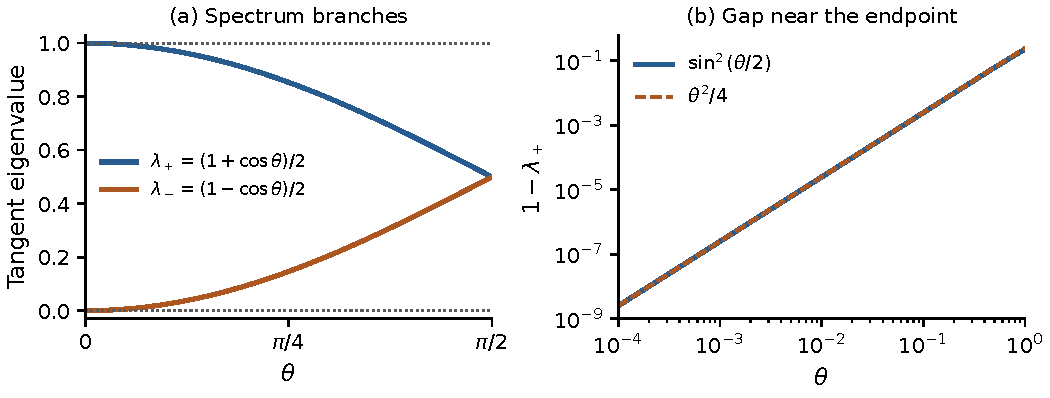
\includegraphics[width=\linewidth]{figures/spectrum.pdf}
\caption{Analytical spectrum from Proposition~\ref{prop:spectrum}. Left: on $0\le\theta\le\pi/2$, the moving branches each have generic multiplicity $8$, while $0$ and $1$ have generic multiplicities $16$ and $32$. Multiplicities combine at the endpoints. Right: the slow-branch gap $1-\lambda_+=\sin^2(\theta/2)$ tends quadratically to zero near $\theta=0$. Curves are sampled from the exact formulas, not fitted eigenvalue data; the dashed curve is the small-angle expression $\theta^2/4$.}
\label{fig:spectrum}
\end{figure}

\section{One-cycle residual obstruction with legal Grams}
\label{sec:obstruction}

The spectrum must be connected to \eqref{eq:residual}, since an eigenvalue of a tangent map alone does not determine an algorithm's stopping observable.

\begin{proposition}
\label{prop:obstruction}
For every $q\in(0,1)$, $\delta\in(0,1)$ and $\eta>0$, there exist $\theta\in(0,\pi/2)$ and $x\in\mathcal C$ such that
\begin{equation}
 0<\fro{x-Q(\theta)}<\eta,\qquad e(F(x))>q\,e(x)>0,
 \label{eq:obstruction}
\end{equation}
and the spectra of all eight Gram matrices inverted in \eqref{eq:cycle} lie in $[1-\delta,1+\delta]$.
\end{proposition}

\begin{proof}
Fix $\theta\in(0,\pi/2)$ and $\lambda=(1+\cos\theta)/2<1$. Proposition~\ref{prop:spectrum} provides a nonzero $E\in\TC(Q)$ with $DF(Q)E=\lambda E$. With $E_i$ the row square of the perturbation and $A_i=A_i(Q)$, define
\begin{equation}
 B_i(E)=E_iA_i\adj+A_iE_i\adj,\qquad
 \alpha=\max_i\fro{B_i(E)}.
 \label{eq:alpha}
\end{equation}
Then $\alpha>0$. Otherwise every $B_i(E)$ vanishes, so $E\in\TR(Q)$ as well. Both tangent projectors fix $E$, giving $DF(Q)E=E$, contrary to $\lambda<1$.

Write the column squares of $E$ as $U_jK_j$, with $K_j\adj=-K_j$. Replace each column square of $Q$ by
\begin{equation}
 U_j(h)=U_j\exp(hK_j),\qquad h\in\R.
 \label{eq:curve}
\end{equation}
The resulting array $x(h)$ is exactly column-unitary and has tangent $E$. The principal-root maps are analytic on positive matrices, so locally
\begin{align}
 x(h)&=Q+hE+O(h^2),\\
 F(x(h))&=Q+h\lambda E+O(h^2),\\
 e(x(h))&=|h|\alpha+O(h^2),\\
 e(F(x(h)))&=|h|\lambda\alpha+O(h^2).
 \label{eq:expansions}
\end{align}
For the residual expansions, each row Gram defect is $hB_i(E)+O(h^2)$. The reverse triangle inequality bounds the difference between its norm and $|h|\fro{B_i(E)}$ by $O(h^2)$. Taking a maximum over four rows preserves that estimate, even if several rows attain the maximum. Therefore
\begin{equation}
 \lim_{h\to0,\,h\ne0}\frac{e(F(x(h)))}{e(x(h))}=\lambda,
 \label{eq:ratio}
\end{equation}
and the denominator is positive for sufficiently small nonzero $h$.

Given $q<1$, choose a positive $\theta$ small enough that $\lambda>q$. For this fixed parameter, take a sufficiently small nonzero $h$ to make the ratio exceed $q$ and the distance smaller than $\eta$. All four initial row Grams and all four post-row column Grams equal $I_4$ at $h=0$. Their spectra vary continuously with $h$. Shrinking $|h|$ further places all eight spectra in $[1-\delta,1+\delta]$ simultaneously and ensures the entire cycle is defined. Since $E\ne0$, the distance is nonzero for sufficiently small nonzero $h$. This proves all stated quantifiers.
\end{proof}

The condition number of each inverted Gram is at most $(1+\delta)/(1-\delta)$, which can approach one. Nevertheless the residual ratio can be arbitrarily close to one along \eqref{eq:curve}, by \eqref{eq:ratio} and $\theta\downarrow0$. Hence no factor $q<1$, independent of the family parameter, can bound $e(F(x))/e(x)$ over these legal nearby inputs. The assertion does not require a neighbourhood radius uniform in $\theta$. It also does not assert that every nonlinear ratio is at most one.

\section{Physical meaning, prior results and limitations}

For an exact array $Q$, its projections $P_{ij}=q_{ij}q_{ij}\adj$ have row and column sums $I_4$. Each fixed row defines the measurement channel
\begin{equation}
 \mathcal M_i(\rho)=\sum_j\Tr(P_{ij}\rho)|j\rangle\langle j|.
 \label{eq:channel}
\end{equation}
The Kraus operators $K_{ij}=|j\rangle\langle q_{ij}|$ satisfy $\sum_jK_{ij}\adj K_{ij}=I_4$. Thus this channel is completely positive and trace preserving, including in the presence of a reference system. Nearby column-unitary witnesses generally have imperfect row completeness and are not exact measurement channels. Nor is $F$ a quantum dynamical channel: it updates classical descriptions of an array.

Our calculation isolates constraint geometry from inverse-Gram conditioning. At the exact family every Gram is $I_4$; the admissible witnesses keep all eight inversions arbitrarily close to that ideal. The poor uniform progress factor comes from the relative row and column tangent spaces. This is useful for checking normalization implementations and for evaluating proposed stopping or rate guarantees. It establishes a local limitation of a conditioning-only guarantee, without prescribing a restart rule or a modified algorithm.

The polar interpretation and related convergence questions predate this calculation \cite[Proposition 5.5 and Conjecture 5.6]{BanicaNechita2017}. Benoist and Nechita prove finite-accuracy termination for a relaxed version with strictly positive definite individual blocks \cite[Appendix A, Proposition A.1]{BenoistNechita2017}. Rank-one blocks $x_{ij}x_{ij}\adj$ in dimension four do not meet that assumption. No uniform regularization limit is supplied here. The known order-four quantum Latin-square examples and their applications \cite{MustoVicary2016} also do not constitute a convergence result for this recurrence.

The general tangent-projector and small-angle mechanism is established in alternating-projection theory \cite{LewisMalick2008}. In the present ambient space, however, both tangent spaces have dimension $64$ and their intersection has positive dimension. Their sum therefore does not have dimension $128$, so ambient transversality fails. An argument based on a clean intersection or a quotient by symmetries would require additional analysis. In particular, the neutral directions counted here are not proved to integrate to a solution manifold.

The original almost-sure arbitrary-precision termination question, all-future inverse legality, nonlinear local convergence and existence of a positive-measure failure basin remain unresolved by these results. One-cycle witnesses do not have to lie in a positive-measure bad basin. Finite iteration caps cannot decide infinite-time termination. The explicit spectrum and source-residual consequence are the claimed contribution; no first-priority assertion is based on a literature search alone.

\section{Reproducible exact calculation}

The analytical block proof establishes both propositions without numerical error. The accompanying symbolic program constructs all tangent generators directly with
\begin{equation}
 t=\tan(\theta/2),\qquad c=\frac{1-t^2}{1+t^2},\qquad
 s=\frac{2t}{1+t^2}.
\end{equation}
It factors the connected-block characteristic polynomials over $\mathbb Q(t)$ and checks a zero exact difference from \eqref{eq:charpoly}. The excluded rational endpoint $\theta=\pi\pmod{2\pi}$ is included in the direct $c,s$ proof. Figure~\ref{fig:spectrum} is regenerated from the exact analytical branches with a standard plotting script. Its samples introduce display roundoff only; they play no role in either proof. The reproduction instructions keep all replay outputs separate from the preserved original scientific inputs.

\section*{Statements and Declarations}

\paragraph{Data and code availability.}
The accompanying local reproducibility package contains the exact generator program, its symbolic output, the analytical-figure script and samples, and build instructions. No experimental or personal data are analyzed. Public archival arrangements remain an author decision.

\paragraph{AI assistance.}
OpenAI Codex language-model assistance was used in literature review, candidate derivations, symbolic and numerical code, automated checking and manuscript drafting. The figure is a deterministic plot of stated analytical formulas. Human scientific, authorship and final-text review has not yet been completed for this local draft. The AI tools are not authors.

\paragraph{Author declarations.}
Funding, competing interests and the supplied author affiliation await confirmation by the human author before submission.

\bibliographystyle{unsrtnat}
\bibliography{references}
\end{document}
